\documentclass[tikz,border=3.14pt]{standalone}
\usepackage{../mymacros}
\usepackage{tikz-3dplot}
\begin{document}
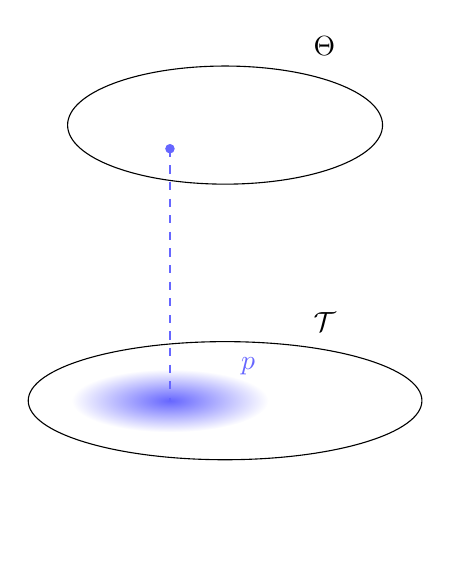
\begin{tikzpicture}[]
\draw[] (0,0,0) ellipse (2 and .75) node[right, shift={(1,1)}]{$\Theta$};
\draw [fill, color=blue!60!white] (-0.7,-0.3,0) circle (1.5pt) node[above](a){$\vtheta$};
\draw[] (0,-3.5,0) ellipse (2.5 and .75) node[right, shift={(1,1)}]{$\mathcal{T}$};
\draw[fill, inner color=blue!60!white, outer color=white, draw=none, color=white] (-0.7,-3.5,0) ellipse (1.25 and .4) node[above, shift={(1,.2)}, color=blue!60!white]{$p_{\vtheta}$};
\draw[dashed, color=blue!60!white] (a) -- (-0.7,-3.5,0);
\phantom{
\draw [fill, color=black] (-1.1,-3.6,0) circle (1.5pt) node[above](b){$\tau$};
\draw[] (-1.1,-5,0) node (c) {$R(\tau)$};
\draw[->] (b) -- (c);
}
\end{tikzpicture}
\end{document}